%% ============================================================
\section{Results}
\label{sec:results}

\subsection{Juliet Benchmark Results}

\Cref{tab:juliet-summary} summarizes SqC v0.4.249's performance on
the Juliet Test Suite in fast mode.

\begin{table}[t]
\centering
\footnotesize
\begin{tabular}{@{}lr@{}}
\toprule
\textbf{Metric} & \textbf{Value} \\
\midrule
Rules implemented & 311 \\
CWEs scanned (fast mode) & 79 \\
Test files & 50,256 \\
True Positives & 22,261 \\
False Positives & 3,121 \\
TP Rate (precision) & 87.7\% \\
Per-file detection rate & 38.0\% \\
100\% precision CWEs & 44 \\
\bottomrule
\end{tabular}
\caption{SqC v0.4.249 Juliet benchmark summary (fast mode).}
\label{tab:juliet-summary}
\end{table}

\subsubsection{Precision Tiers}

The 79 CWEs tested fall into five tiers, shown in
\cref{tab:precision-tiers}.  The distribution is encouraging: the
44 CWEs at 100\% precision and the 22 at high precision together are
84\% of scored CWEs, and no CWE falls below 33\%; the 12 zero-detection
CWEs (rules mapped to them but no Juliet testcase triggers a finding)
are a distinct category from low precision, not a failure mode.

\begin{table}[t]
\centering
\footnotesize
\begin{tabular}{@{}lrrr@{}}
\toprule
\textbf{Tier} & \textbf{CWEs} & \textbf{TP Rate} & \textbf{TP} \\
\midrule
100\% Precision & 44 & 100\% & 9,835 \\
High ($>$50\%) & 22 & 50--99\% & 12,418 \\
Medium (33--50\%) & 1 & 33--50\% & 8 \\
Low ($<$33\%) & 0 & --- & 0 \\
Zero Detection & 12 & --- & 0 \\
\midrule
\textbf{Total} & \textbf{79}\textsuperscript{$\dagger$} & & \textbf{22,261} \\
\bottomrule
\end{tabular}
\caption{CWE distribution by precision tier (fast mode, v0.4.249).
\textsuperscript{$\dagger$}All 79 scanned CWEs; the 12 with zero
detection contribute 0 TP.}
\label{tab:precision-tiers}
\end{table}

\Cref{tab:perfect-cwes} lists the 44 CWEs with 100\% precision (out of
79 scanned; a further 12 are mapped rules with zero Juliet detections
rather than false positives).  These represent vulnerability classes
where SqC produces zero false positives on Juliet---every reported
violation is a true defect on this benchmark.  Notably, CWE-190
(integer overflow) joined this list with the opt-in provenance-gated
rewrite of the INT rules (\cref{sec:provenance-frontier}), which
eliminated its remaining Juliet false positives as a side effect of the
real-world-motivated redesign.

A 100\% Juliet precision figure is a claim about the synthetic
benchmark only, not a guarantee that generalizes to real-world code.
CWE-690 is the clearest cautionary case: 100\% on Juliet
(\cref{tab:perfect-cwes}) but 0.66\% on the adjudicated real-world
oracle (\cref{sec:realworld-results}). CWE-78 (ENV33-C, ENV03-C,
STR02-C) has not received the same breadth of real-world auditing---only
12 labeled findings, all from raylib---but even that thin sample is
inconsistent across the three contributing rules: ENV33-C is 4/4 TP,
while ENV03-C and STR02-C are 0/4 TP (all FP). We report the Juliet
number as measured and do not claim it generalizes; readers should
weight per-CWE 100\% figures by the corresponding real-world evidence
in \cref{sec:realworld-results} where available, and treat CWEs
without that evidence (like CWE-78) as unvalidated rather than
confirmed.

\begin{table}[t]
\centering
\footnotesize
\begin{tabular}{@{}lrr@{}}
\toprule
\textbf{CWE} & \textbf{Description} & \textbf{TP} \\
\midrule
CWE-78  & OS Command Injection & 2,810 \\
CWE-190 & Integer Overflow & 1,498 \\
CWE-690 & Null Deref from Return & 558 \\
CWE-195 & Signed to Unsigned Conversion & 520 \\
CWE-197 & Numeric Truncation Error & 468 \\
CWE-253 & Incorrect Check of Return Value & 432 \\
CWE-680 & Int Overflow $\to$ Buffer Overflow & 352 \\
CWE-758 & Reliance on Undefined Behavior & 342 \\
CWE-194 & Unexpected Sign Extension & 310 \\
CWE-761 & Free Pointer Not at Start & 276 \\
CWE-563 & Unused Variable & 272 \\
CWE-590 & Free Memory Not on Heap & 240 \\
CWE-789 & Uncontrolled Mem Alloc & 190 \\
CWE-398 & Indicator of Poor Code Quality & 162 \\
\multicolumn{2}{@{}l}{\emph{+ 30 more CWEs}} & 1,405 \\
\midrule
\textbf{Total} & & \textbf{9,835} \\
\bottomrule
\end{tabular}
\caption{CWEs with 100\% precision (zero false positives), v0.4.249.}
\label{tab:perfect-cwes}
\end{table}

\subsubsection{Top Rules by Detection Volume}

\Cref{tab:top-rules} shows the 10 rules contributing the most true
positives.  These rules account for 67\% of all TPs.  The FP rates
vary significantly: EXP34-C achieves 13\% FP rate (CFG-based null-state
dataflow), while ARR30-C is at 28\% (buffer size estimation without
full alias analysis).  ENV33-C, INT32-C, INT31-C, and ENV03-C now
achieve 0\% FP rate; INT32-C and INT31-C reached zero-FP as a direct
result of the opt-in provenance-gated rewrite discussed in
\cref{sec:provenance-frontier}, which trades some Juliet recall (fewer
TP than the v0.4.22 figures) for eliminating essentially all of their
FPs on both benchmarks.  FIO30-C's FP rate dropped sharply since
v0.4.116 (11\%$\to$1.8\%) from a round of cross-translation-unit and
function-pointer format-string false-positive fixes
(\cref{fig:tp-rate-progression}).

\begin{table}[t]
\centering
\footnotesize
\begin{tabular}{@{}lrrrl@{}}
\toprule
\textbf{Rule} & \textbf{TP} & \textbf{FP} & \textbf{FP\%} & \textbf{Primary CWEs} \\
\midrule
INT32-C & 2,425 & 0    & 0  & 190, 191, 680 \\
ARR38-C & 2,142 & 648  & 23 & 121, 126, 124 \\
ARR30-C & 1,803 & 699  & 28 & 121, 122, 126 \\
FIO30-C & 1,650 & 30   & 2  & 134 \\
STR31-C & 1,608 & 278  & 15 & 121, 122, 124 \\
ENV33-C & 1,550 & 0    & 0  & 78 \\
INT31-C & 1,070 & 0    & 0  & 195, 194, 197 \\
EXP33-C & 914   & 35   & 4  & 457, 758, 665 \\
EXP34-C & 850   & 127  & 13 & 690, 476 \\
ENV03-C & 832   & 0    & 0  & 78, 426 \\
\bottomrule
\end{tabular}
\caption{Top 10 rules by true positive volume (fast mode, v0.4.249).}
\label{tab:top-rules}
\end{table}

\subsubsection{TP Rate Progression}

\Cref{fig:tp-rate-progression} shows the TP rate progression across
the project's development history.  The full-suite baseline started at
41.1\% (v0.2.1); after 12 rounds of FP reduction, it reached 44.6\%
(v0.2.25).  The switch to fast-mode benchmarking (v0.3.20) established
a new baseline of 45.8\%, which improved to 72.7\% by v0.4.22 through
value-range analysis, CFG constant resolution, cross-function taint
tracking, and targeted per-CWE FP reduction.  Progress continued past
v0.4.22: the opt-in provenance-gated INT rewrite
(\cref{sec:provenance-frontier}, v0.4.38) and subsequent per-rule
tuning pushed the rate to 83.2\% by v0.4.46, after which it plateaued
--- v0.4.116 sits at 83.8\%, within 0.6 points of the v0.4.46 figure
despite dozens of intervening releases, consistent with the
diminishing-returns pattern of \cref{sec:fp-reduction}. The plateau
continues through v0.4.175 (85.5\%): a soundness fix to MEM30-C's
branch-merge logic (a stale-nullified-state bug that had been
silently masking real use-after-free/double-free hits since before
v0.4.116, unrelated to any FP-reduction effort) recovered
CWE-416's TP rate from 86.7\% to 91.3\% and CWE-415's from 58.6\% to
62.8\% at zero added false positives, but because both CWEs are a
small share of the full 79-CWE suite, the aggregate move is only
+0.1 points (85.4\%$\to$85.5\%) --- a reminder that a real,
zero-cost correctness fix can be nearly invisible in an aggregate
rate dominated by high-volume CWEs.

A methodological note applies to both the v0.4.175 and v0.4.249
points: v0.4.139 (between v0.4.116 and v0.4.175, not separately
plotted) enabled 15 of 21 previously-untracked CERT-C rules
surfaced by a wiki re-ingest that had never been implemented before.
Three of the 15 map to CWEs already present in the Juliet suite ---
MSC00-C (CWE-563/570/571), MSC11-C (CWE-190), and MSC24-C
(CWE-197/367/464/676/242; CWE-114 was later dropped from its mapping)
--- so some of the movement at v0.4.175 and v0.4.249 reflects newly
enabled rule coverage rather than fixes to pre-existing rules alone.
MSC11-C's CWE-190 hits in particular overlap with INT32-C/INT30-C's
pre-existing detections on the same files and should not be read as
net-new coverage without confirming they are not duplicate flags on
cases the two established rules already caught.

The plateau breaks decisively at v0.4.249 (87.7\%, +2.2 points over
v0.4.175), the largest single jump since v0.4.46. Unlike the v0.4.175
point, this was not one isolated fix but a scoping-and-deduplication
pass across the buffer-size-resolution subsystem shared by ARR30-C,
ARR38-C, and STR31-C (consolidating three independently-drifted
size-inference implementations onto one shared \texttt{buffer\_size.rs}
module, and fixing several cross-function variable-name-conflation
bugs where a same-named buffer in a different function was credited
with the wrong size) plus a cross-translation-unit and
function-pointer fix to FIO30-C's format-string tracking. The net
effect over this window (\texttt{bench compare v0.4.175 v0.4.249}) is
$+329$ TP and $-590$ FP; the two largest movers are CWE-121/CWE-122
(stack/heap buffer overflow, $-76$/$-80$ FP with $+258$/$+115$ TP from
the buffer-size fixes recovering previously-missed real detections
alongside removing false ones) and CWE-134 (format string, $-180$ FP
from the FIO30-C fix, TP unchanged). CWE-369 (divide by zero) moved
the other way on this pass ($-132$ FP but also $-104$ TP), a reminder
that not every FP-reduction round is free even when the aggregate
trend is positive.

\begin{figure}[t]
\centering
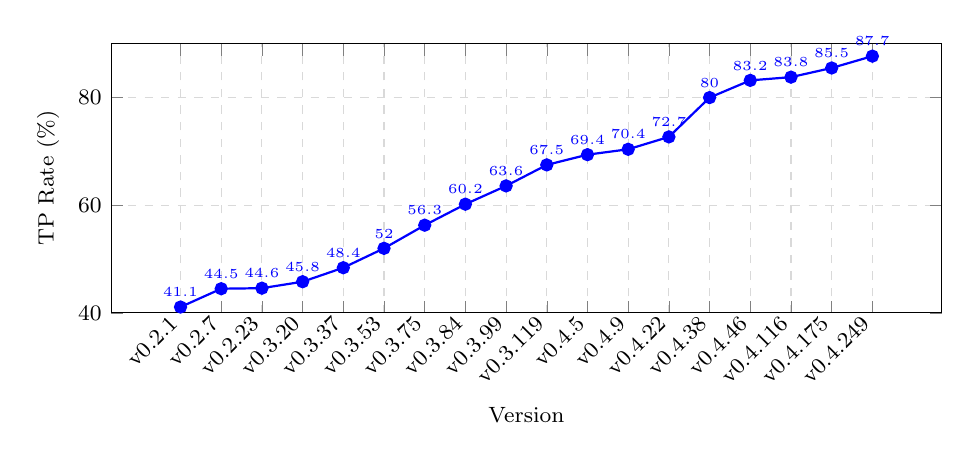
\begin{tikzpicture}
\begin{axis}[
    width=\columnwidth,
    height=5cm,
    xlabel={Version},
    ylabel={TP Rate (\%)},
    ymin=40, ymax=90,
    xtick=data,
    xticklabels={v0.2.1, v0.2.7, v0.2.23, v0.3.20, v0.3.37, v0.3.53, v0.3.75, v0.3.84, v0.3.99, v0.3.119, v0.4.5, v0.4.9, v0.4.22, v0.4.38, v0.4.46, v0.4.116, v0.4.175, v0.4.249},
    xticklabel style={rotate=45, anchor=east, font=\footnotesize},
    ylabel style={font=\footnotesize},
    xlabel style={font=\footnotesize},
    tick label style={font=\footnotesize},
    nodes near coords,
    nodes near coords style={font=\tiny},
    every node near coord/.append style={anchor=south},
    grid=major,
    grid style={dashed, gray!30},
]
\addplot[color=blue, mark=*, thick] coordinates {
    (1, 41.1) (2, 44.5) (3, 44.6) (4, 45.8) (5, 48.4) (6, 52.0) (7, 56.3) (8, 60.2) (9, 63.6) (10, 67.5) (11, 69.4) (12, 70.4) (13, 72.7) (14, 80.0) (15, 83.2) (16, 83.8) (17, 85.5) (18, 87.7)
};
\end{axis}
\end{tikzpicture}
\caption{TP rate progression from baseline (v0.2.1) through current
(v0.4.249).  The gap between v0.2.23 and v0.3.20 reflects the switch
from full-suite to fast-mode benchmarking.  The rate plateaus after
v0.4.46 despite continued FP-reduction work, reflecting the
diminishing-returns dynamic of \cref{sec:fp-reduction}.  The v0.4.175
point reflects a MEM30-C soundness fix that recovered CWE-416/415 TP
rate by 4--5 points each at zero added FP, but moves the aggregate
rate by only +0.1 points since both CWEs are a small share of the
79-CWE suite.  The plateau breaks at v0.4.249 (+2.2 points), driven by
a shared buffer-size-resolution consolidation across ARR30-C/ARR38-C/
STR31-C and a FIO30-C format-string fix (CWE-121/122/134 are the
largest movers); this is the largest single-version gain since
v0.4.46.  Between v0.4.116 and v0.4.175 (not separately plotted),
v0.4.139 enabled 15 previously-untracked rules, three of which
(MSC00-C, MSC11-C, MSC24-C) overlap existing Juliet CWEs; the
v0.4.175/v0.4.249 points are not purely FP-reduction movement (main
text).}
\label{fig:tp-rate-progression}
\end{figure}

\subsection{Competitor Comparison}
\label{sec:competitor}

\Cref{tab:competitor} compares SqC against four open-source tools on 15
overlapping Juliet CWEs.  All tools were run on the same test files with
TP/FP classified using identical Juliet ground truth (procedure names
and \texttt{OMITBAD}/\texttt{OMITGOOD} guards).

\begin{table*}[t]
\centering
\footnotesize
\setlength{\tabcolsep}{4pt}
\begin{tabular}{@{}llrrrrr@{}}
\toprule
\textbf{CWE} & \textbf{Description} & \textbf{SqC} & \textbf{cppcheck} & \textbf{clang-tidy} & \textbf{Infer} & \textbf{Frama-C} \\
\midrule
121 & Stack Buffer Overflow       & 74.8 & 40.5 & \textbf{86.6} & 38.8 & --- \\
122 & Heap Buffer Overflow        & 83.7 & 45.0 & \textbf{89.5} & 37.8 & --- \\
124 & Buffer Underwrite           & 70.9 & 40.5 & \textbf{90.4} & 33.9 & --- \\
127 & Buffer Underread            & 87.8 & 42.7 & \textbf{93.2} & 33.9 & --- \\
190 & Integer Overflow            & \textbf{100.0} & 27.5 & 94.3 & --- & 58.1 \\
191 & Integer Underflow           & \textbf{98.5} & 27.2 & 94.4 & --- & 63.1 \\
197 & Numeric Truncation          & \textbf{100.0} & 40.0 & 94.5 & --- & \textbf{100.0} \\
369 & Divide by Zero              & 61.4 & 27.4 & \textbf{94.7} & --- & 43.4 \\
401 & Memory Leak                 & 78.0 & 25.7 & \textbf{83.9} & 54.7 & --- \\
415 & Double Free                 & 62.8 & 33.8 & \textbf{80.0} & 63.0 & --- \\
416 & Use After Free              & \textbf{91.3} & 29.6 & 60.3 & 2.0  & --- \\
476 & Null Pointer Deref          & 67.9 & 39.7 & \textbf{94.3} & 66.1 & 64.2 \\
680 & Int Overflow $\to$ BOF      & \textbf{100.0} & 40.8 & 95.9 & --- & 82.6 \\
690 & Null Deref from Return      & \textbf{100.0} & 45.7 & 88.0 & 60.0 & --- \\
761 & Free Not at Start           & \textbf{100.0} & 45.7 & 94.3 & 58.1 & --- \\
\midrule
\multicolumn{2}{@{}l}{\textbf{Overall TP rate}} & 82.6 & 36.4 & \textbf{91.6} & 43.6 & 61.0 \\
\multicolumn{2}{@{}l}{\textbf{CWEs tested}}     & \textbf{79} & 15 & 15 & 10 & 6 \\
\bottomrule
\end{tabular}
\caption{TP rate (\%) comparison on overlapping Juliet CWEs.
\textbf{Bold} = highest per row.  ``---'' = CWE not tested by that tool.
SqC v0.4.271; cppcheck 2.10; clang-tidy (LLVM 21.1); Infer v1.2.0; Frama-C 32.0 EVA.
Competitor numbers are held fixed from the original study (not
re-measured); SqC's column reflects v0.4.271.
All tools run on same test files (28{,}488 total across 15 CWEs).}
\label{tab:competitor}
\end{table*}

Four patterns persist in this refreshed snapshot, which updates SqC's
column from v0.4.116 to v0.4.271 (155 releases, mostly real-world
FP-reduction work per \cref{sec:fp-reduction} rather than
Juliet-targeted tuning); the competitor columns are unchanged, held
fixed from the original study.  First, \textbf{clang-tidy still
achieves the highest overall precision} (91.6\%) with only 116 false
positives across all 15 CWEs, but the gap has continued to narrow:
SqC's overall rate on these 15 CWEs is now 82.6\% (up from 79.5\% at
v0.4.116, 68.2\% at the original snapshot), and it detects far more
total violations than clang-tidy (22{,}261 vs.\ 13{,}952 TP, though
note SqC's figure is summed over all 79 CWEs it tests, not just these
15).

Second, \textbf{SqC still beats clang-tidy outright on the same six
CWEs it won at v0.4.116}: CWE-190 (100.0\% vs.\ 94.3\%), CWE-191
(98.5\% vs.\ 94.4\%), CWE-416 (91.3\% vs.\ 60.3\%), CWE-680 (100.0\%
vs.\ 95.9\%), CWE-690 (100.0\% vs.\ 88.0\%), and CWE-761 (100.0\% vs.\
94.3\%), plus ties Frama-C at 100.0\% on CWE-197.  None of the 155
intervening releases flipped a row's winner in either direction; the
movement on the other nine rows is incremental (e.g.\ CWE-121 74.8\%
vs.\ 71.0\%, CWE-369 61.4\% vs.\ 57.8\%, CWE-415 62.8\% vs.\ 57.6\%)
rather than structural, consistent with the plateau-then-real-world-fix
pattern described in \cref{sec:fp-reduction} --- none of that work
targeted these 15 CWEs specifically.

Third, \textbf{SqC has further extended its lead over Frama-C}: 82.6\%
vs.\ Frama-C's 61.0\% on the 15 overlapping CWEs (was 79.5\% vs.\
61.0\% at v0.4.116, 68.2\% vs.\ 61.0\% at the original snapshot), while
covering 79 CWEs vs.\ Frama-C's 6.  SqC still exceeds Frama-C on
CWE-369 (61.4\% vs.\ 43.4\%), CWE-190 (100.0\% vs.\ 58.1\%), CWE-191
(98.5\% vs.\ 63.1\%), and CWE-680 (100.0\% vs.\ 82.6\%).

Fourth, \textbf{SqC wins on six CWEs outright}: CWE-190, CWE-680,
CWE-690, and CWE-761 at 100\%, CWE-191 at 98.5\%, and CWE-416
use-after-free (91.3\% vs.\ clang-tidy's 60.3\%), where MEM01-C's
flow-sensitive deref tracking after \texttt{free} distinguishes the
good/bad paths more reliably than clang-tidy's pattern checks.
CWE-416 has recovered slightly since v0.4.116 (90.7\%) and sits just
below the 92.9\% figure from the original study; it remains the clear
leader on this CWE regardless.

Fifth, \textbf{cppcheck still produces the most findings but the lowest
precision} (36.4\%), reflecting its heuristic approach.  Its 29{,}377
TPs represent high recall but at the cost of 51{,}361 FPs.

The coverage gap remains the key differentiator: SqC tests 79 CWEs
spanning 17 CERT~C categories, while the other tools cover 6--15 on
this benchmark.  A hypothetical ensemble of all five tools would
achieve both high per-CWE precision and broad coverage.

\subsection{Real-World Results}
\label{sec:realworld-results}

\Cref{tab:realworld-results} compares SqC against cppcheck and
clang-tidy across the 9-project real-world set. seL4 has no
cppcheck/clang-tidy baseline yet (onboarded as a ninth oracle after the
last competitor sweep); sqlite's scan scope narrowed between versions
(125$\to$81 in-scope files) as its file predicate was tightened, not a
regression.

\begin{table}[t]
\centering
\footnotesize
\begin{tabular}{@{}lrrr@{}}
\toprule
\textbf{Project} & \textbf{sqc} & \textbf{cppcheck} & \textbf{clang-tidy} \\
\midrule
libcrc & 395 & 40 & 2 \\
lua & 3,047 & 49 & 107 \\
raylib & 4,749 & 1,060 & 469 \\
mosquitto & 2,970 & 277 & 44 \\
curl & 8,582 & 556 & 116 \\
sqlite & 18,922 & 503 & 137 \\
hostap & 30,752 & 1,761 & 1,710 \\
pure-ftpd & 5,855 & 12 & 109 \\
seL4 & 4,959 & --- & --- \\
\midrule
\textbf{Total} & \textbf{80,231} & \textbf{4,258} & \textbf{2,694} \\
\bottomrule
\end{tabular}
\caption{Violation counts (sqc v0.4.249, cppcheck v2.10, clang-tidy
v21.1.6).  Excluding seL4 (no competitor baseline), SqC's total is
75,272 across the other 8 projects --- an $\sim$18--28$\times$
difference vs.\ cppcheck/clang-tidy, reflecting SqC's 311-rule coverage
vs.\ $\sim$20 checks in competitors.  SqC's own total dropped 28\% from
the v0.4.120 figure (104,733 across the original 7 projects) despite
covering more rules, from the FP-reduction work in
\cref{sec:fp-reduction} landing on real-world code, not just Juliet.}
\label{tab:realworld-results}
\end{table}

Beyond raw violation volume, what matters is what fraction of these
findings are real: scored against a hand-adjudicated ground-truth
oracle spanning all 9 projects (\cref{sec:ground-truth-snapshot}), aggregate
measured precision is 16.6\% (TP 10,561 of 63,608 labeled findings) with
97.4\% recall (10,561 of 10,841 known true positives flagged), at 86.3\%
label coverage (63,649 of 73,718 total findings labeled;
run \texttt{sqc-0.4.258}). As with the Juliet 100\%-precision figures
in \cref{tab:perfect-cwes}, this aggregate number should be read scoped
to its oracle rather than as a universal precision claim
(\cref{sec:limitations}).

\Cref{tab:realworld-timing} reports analysis throughput.  Each tool was
run serially---one process at a time, with the full machine to itself---so
the durations are uncontended wall-clock process runtime; throughput is
LOC divided by that runtime.  LOC is physical lines over the same curated
source scope used as the denominator for all three tools.

\begin{table}[t]
\centering
\footnotesize
\setlength{\tabcolsep}{4pt}
\resizebox{\columnwidth}{!}{%
\begin{tabular}{@{}lrrrr@{}}
\toprule
& & \multicolumn{3}{c}{\textbf{Time (s) / Throughput (LOC\,s$^{-1}$)}} \\
\cmidrule(l){3-5}
\textbf{Project} & \textbf{LOC} & \textbf{sqc} & \textbf{cppcheck} & \textbf{clang-tidy} \\
\midrule
libcrc & 1,034 & 0.6 / 1,723 & 0.1 / 10,340 & 0.1 / 10,340 \\
mosquitto & 39,368 & 22.6 / 1,741 & 3,278.8 / 12 & 2.3 / 17,116 \\
curl & 186,220 & 72.5 / 2,568 & 642.5 / 289 & 4.8 / 38,795 \\
sqlite & 218,733 & 165.5 / 1,321 & 1,198.7 / 182 & 7.0 / 31,247 \\
hostap & 589,724 & 353.1 / 1,670 & 2,659.3 / 221 & 55.9 / 10,549 \\
\bottomrule
\end{tabular}}
\caption{Real-world analysis time and throughput (sqc v0.4.55,
cppcheck v2.10, clang-tidy v21.1.6), measured serially to avoid CPU
contention.  SqC throughput is stable at $\sim$1{,}300--2{,}600\,LOC\,s$^{-1}$
across codebases.  cppcheck is intrinsically slow---54.6\,min on
mosquitto (12\,LOC\,s$^{-1}$) despite its small size---rather than
contention-bound.  clang-tidy is fastest here but runs a narrower check
set (cf.~its violation counts in \cref{tab:realworld-results}), so its
throughput is not directly comparable on analysis depth.  This table has
not been re-measured since v0.4.55: the automated benchmark harness now
runs projects concurrently for throughput, so its per-run duration
figures (\cref{sec:realworld-results}) are not directly comparable to
the strict single-process, uncontended protocol this table requires.
A fresh controlled re-measurement at the current version is future work;
the per-CWE scan-time trend below (\cref{fig:scan-time}), which is
contention-independent by construction, is the up-to-date proxy for
how analysis cost has evolved since v0.4.55.}
\label{tab:realworld-timing}
\end{table}

\Cref{fig:realworld-reduction} shows that FP reductions developed on
Juliet transfer to real-world code in the aggregate: total violations
across the original five codebases dropped 82.4\% from v0.2.7 to
v0.4.120, though nearly all of that reduction had already landed by
v0.4.22 --- the subsequent 98 releases removed a further 27.7\% on top
of the v0.4.22 figure, another instance of the diminishing-returns
pattern (\cref{fig:tp-rate-progression}).
(\Cref{sec:limitations} shows the important caveat: aggregate volume
reduction does not imply real-world precision.)

\begin{figure}[t]
\centering
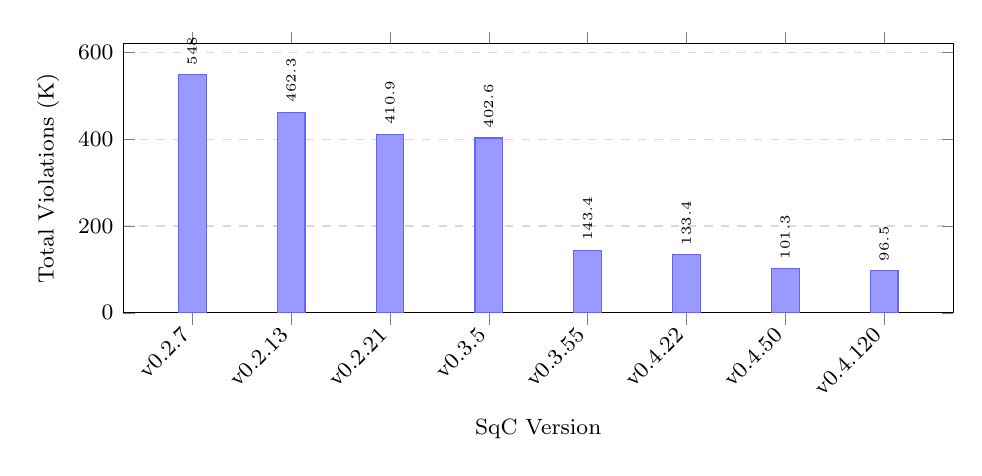
\begin{tikzpicture}
\begin{axis}[
    width=\columnwidth,
    height=5cm,
    ybar,
    xlabel={SqC Version},
    ylabel={Total Violations (K)},
    ymin=0, ymax=620,
    xtick=data,
    xticklabels={v0.2.7, v0.2.13, v0.2.21, v0.3.5, v0.3.55, v0.4.22, v0.4.50, v0.4.120},
    xticklabel style={rotate=45, anchor=east, font=\footnotesize},
    ylabel style={font=\footnotesize},
    xlabel style={font=\footnotesize},
    tick label style={font=\footnotesize},
    bar width=10pt,
    nodes near coords,
    nodes near coords style={font=\tiny, rotate=90, anchor=west},
    ymajorgrids=true,
    grid style={dashed, gray!30},
]
\addplot[fill=blue!40, draw=blue!60] coordinates {
    (1, 548.0)
    (2, 462.3)
    (3, 410.9)
    (4, 402.6)
    (5, 143.4)
    (6, 133.4)
    (7, 101.3)
    (8, 96.5)
};
\end{axis}
\end{tikzpicture}
\caption{Total SqC violations across the original 5 real-world
codebases by version (libcrc, mosquitto, curl, sqlite, hostap; lua and
raylib excluded here for continuity with the pre-v0.4.83 series).
Reduction v0.2.7$\to$v0.4.120: $-$451,506 ($-$82.4\%).}
\label{fig:realworld-reduction}
\end{figure}

For the one rule where all three tools have overlapping coverage
(null pointer dereference), the difference in analysis philosophy is
stark.  On mosquitto, SqC reports 386 EXP34-C violations at v0.4.120
(down from 8,657 at v0.3.5, and further down from 504 at v0.4.22)
compared to cppcheck's 2 \texttt{nullPointer} findings.  cppcheck fires
only when it can \emph{prove} a null dereference path exists; SqC flags
all paths that \emph{may} dereference a null pointer.  This is a
fundamental tradeoff between coverage and precision that different
users will weight differently, and the adjudicated oracle
(\cref{sec:limitations}) quantifies its cost: even after a
22$\times$ volume reduction, EXP34-C's measured precision across the
six audited projects (curl, hostap, lua, mosquitto, raylib, sqlite) is
0.66\% (15 TP / 2{,}264 labeled), so the overwhelming majority of
EXP34-C findings on real-world code are still false positives ---
starkly at odds with CWE-690's 100\% precision on Juliet
(\cref{tab:perfect-cwes}); EXP34-C also covers CWE-476, so its own
Juliet-wide FP rate is a more modest 13\% (\cref{tab:top-rules}), but
even that headline number does not survive contact with real-world
code.

That low precision coexists with a concentrated pocket of confirmed
true positives.  Delta-adjudicating EXP34-C's findings against
SQLite's \texttt{ext/} extension modules --- code reachable only
through optional loadable extensions, and correspondingly less
scrutinized than the core engine --- confirmed 11 genuine
out-of-memory-triggered NULL-dereference bugs: an unchecked
\texttt{sqlite3\_malloc64()} result used directly in \texttt{fread()}
(\texttt{ext/expert/expert.c}); \texttt{sqlite3\_column\_name()}
strlen'd with no NULL check at two sites in
\texttt{ext/fts3/fts3.c}; \texttt{sqlite3\_column\_text()} indexed and
compared with no NULL check in \texttt{ext/misc/amatch.c} (SQL-NULL
triggerable, not merely OOM); \texttt{sqlite3\_vmprintf()} consumed
unguarded at two sites in \texttt{ext/misc/sqlite3\_stdio.c};
\texttt{sqlite3\_stmt\_scanstatus\_v2()}'s
\texttt{SQLITE\_SCANSTAT\_EXPLAIN} output used unguarded on its normal
(non-error) return path in \texttt{ext/qrf/qrf.c}; and an
\texttt{sqlite3\_mprintf()} result passed to plain libc \texttt{printf}'s
\texttt{\%s} --- bypassing SQLite's own NULL-safe \texttt{mprintf} ---
in \texttt{ext/session/changeset.c}.  Cross-checking against the live
upstream mainline found 4 of the original 11 sites already
independently hardened by a June 2026 OOM-hardening pass; we filed
disclosures for the remaining six, covering
\texttt{expert.c}\footnote{\url{https://sqlite.org/bugs/forumpost/c06a3c0d3f}},
\texttt{amatch.c}\footnote{\url{https://sqlite.org/bugs/forumpost/20d89d613b}},
\texttt{sqlite3\_stdio.c}\footnote{\url{https://sqlite.org/bugs/forumpost/ba00fdddda}},
\texttt{changeset.c}\footnote{\url{https://sqlite.org/bugs/forumpost/f20ea456ac}},
\texttt{fts3.c}\footnote{\url{https://sqlite.org/bugs/forumpost/9b4276628a}},
and \texttt{qrf.c}\footnote{\url{https://sqlite.org/bugs/forumpost/18338dc19d}}.
SQLite fixed all six the same day they were filed, extending the
same-day/next-day turnaround documented in
\cref{sec:provenance-frontier} to nine consecutive disclosures across
this evaluation.  Unlike the \texttt{kvvfsDecode} finding in
\cref{sec:provenance-frontier} (an audit-discovered false negative,
not a rule detection), these 11 sites are genuine EXP34-C true
positives --- the rule flagged real bugs, adjudication confirmed them
against source, and the resulting disclosures were externally
validated by the same-day fixes.  They are a small fraction of
EXP34-C's real-world output, but a concrete demonstration that its
0.66\% measured precision reflects volume of false alarms, not an
absence of genuine findings underneath them.

\subsection{A Defect Class Juliet Cannot Surface}
\label{sec:juliet-blindspot}

The precision gap above is the expected direction of disagreement:
Juliet flatters a rule that misbehaves in the field.  The real-world
oracles also disagree in the \emph{opposite} direction---they expose
defects in the analyzer that Juliet structurally cannot report at all.
The clearest case is a class of duplicate-finding bugs, where a rule
emits the same diagnostic more than once for a single program fact.

A complete adjudication of our fifth oracle, Lua~5.5
(\texttt{lgc.c}~@\,\texttt{40b76de2}), surfaced the severe form.  DCL02-C
(visually similar identifiers) re-emitted the identical \texttt{n}/\texttt{h}
diagnostic 100~times on each of two source lines: 200 of the rule's
203 findings on that file were exact duplicates of just two real
diagnostics (\cref{tab:dup-class}).  The root cause was an
$O(\text{depth})$ re-traversal---the rule re-analyzed each enclosing
block, re-emitting once per pairwise comparison rather than once per
declaration site---so the duplication factor scales with block-nesting
depth.  Juliet never surfaced this: its synthetic test cases are small
and shallow, and none reaches the nesting depth at which the blow-up
becomes visible.

Prompted by that finding, we audited the same bug \emph{class} across
the rule set and found milder, constant-factor instances whose inputs
\emph{were} present in Juliet: POS37-C emitted every dropped-privilege
finding twice (2.0$\times$, all CWE273 cases), SIG31-C emitted some
shared-object accesses twice (1.5$\times$, CWE364), and FIO42-C reported
one resource under two mutually exclusive messages---unclosed
\texttt{FILE*} \emph{and} unclosed file descriptor---a misclassification
inflating CWE404 by 1.53$\times$.  Crucially, Juliet's pass/fail oracle
could not flag even these: a Juliet \texttt{bad} case passes when the
finding set for the seeded defect is non-empty, so a duplicated or
misclassified finding scores identically to a single correct one.  The
metric is count-blind by construction; the defects were latent in the
Juliet corpus but invisible to its scoring.

\begin{table}[t]
\centering
\footnotesize
\setlength{\tabcolsep}{4pt}
\begin{tabular}{@{}llrl@{}}
\toprule
\textbf{Rule} & \textbf{Surfaced by} & \textbf{Factor} & \textbf{Mechanism} \\
\midrule
DCL02-C & Lua (real-world)  & 100$\times$  & $O(\text{depth})$ re-traversal \\
POS37-C & Juliet CWE273     & 2.0$\times$  & subtree visited twice \\
SIG31-C & Juliet CWE364     & 1.5$\times$  & per-reference emit \\
FIO42-C & Juliet CWE404     & 1.53$\times$ & opener misclassification \\
\bottomrule
\end{tabular}
\caption{Duplicate-finding defects.  DCL02-C's scale-dependent form
(200 of 203 \texttt{lgc.c} findings were duplicates of two lines) was
reachable only through real-world depth; the constant-factor forms were
present in Juliet inputs but invisible to its presence-based oracle.
All four are fixed at the rule level (v0.4.58--v0.4.63).}
\label{tab:dup-class}
\end{table}

These are two distinct blind spots, and the real-world oracle covers
both.  The first is one of \emph{scale}: synthetic micro-benchmarks do
not exercise the depth, size, and idiom at which structural or
algorithmic defects manifest.  The second is one of \emph{oracle
granularity}: a presence-based pass/fail metric cannot detect
over-emission at any scale, whereas the real-world audit counts and
inspects every individual finding.  This is direct evidence that the
six real-world oracles complement Juliet rather than duplicate it:
they measure deployment precision (\cref{sec:limitations}), and they
exercise the analyzer at a scale and granularity Juliet does not reach.

\subsection{Runtime Performance}
\label{sec:runtime}

To characterize SqC's runtime behavior across hardware configurations,
we ran single-process scans (cross-file analysis enabled, no prescan
cache) on four machines (\cref{tab:testbed}).

\begin{table}[t]
\centering
\footnotesize
\begin{tabular}{@{}clccc@{}}
\toprule
\textbf{ID} & \textbf{CPU} & \textbf{Cores} & \textbf{RAM} & \textbf{Disk} \\
\midrule
M1 & Xeon E5-2640 @ 2.50\,GHz & 6/24 & 192\,GB & SSD \\
M2 & Ryzen 5 PRO 2400GE @ 3.20\,GHz & 4/8  & 16\,GB  & SSD \\
M3 & i7-7700T @ 2.90\,GHz    & 4/8  & 16\,GB  & SSD \\
M4 & i7-9750H @ 2.60\,GHz    & 6/12 & 16\,GB  & HDD \\
\bottomrule
\end{tabular}
\caption{Test machines.  Cores listed as physical/logical.
All run Linux 6.x.  M1 is a rack server; M2--M4 are desktop/laptop
class.}
\label{tab:testbed}
\end{table}

\Cref{tab:runtime} shows wall-clock times for single-process analysis
of sqlite (404K LOC) across all four machines with cross-file analysis
enabled and no prescan cache (cold start).

\begin{table}[t]
\centering
\footnotesize
\begin{tabular}{@{}crr@{}}
\toprule
\textbf{Machine} & \textbf{Time (s)} & \textbf{LOC/s} \\
\midrule
M1 & 3{,}470 & 117 \\
M2 & 3{,}116 & 130 \\
M3 & 2{,}363 & 171 \\
M4 & 1{,}986 & 204 \\
\bottomrule
\end{tabular}
\caption{Single-process analysis time for sqlite (404,701 LOC,
cross-file analysis enabled, cold cache).}
\label{tab:runtime}
\end{table}

\textbf{Scaling across codebases.}
\Cref{tab:runtime-scaling} shows how throughput varies with codebase
size on M1.  Throughput generally decreases for larger codebases
because cross-file analysis cost grows with the number of
inter-procedural edges.  The exception is sqlite, whose throughput
(117 LOC/s) is lower than the larger hostap (155 LOC/s).  This is
because sqlite ships as a single 230K-line amalgamation file
(\texttt{sqlite3.c}) with dense internal cross-references, whereas
hostap distributes its code across 504 files averaging $\sim$1{,}070
LOC each.  Per-file analysis cost is dominated by intra-file
complexity, not total codebase size.

\begin{table}[t]
\centering
\footnotesize
\begin{tabular}{@{}lrrr@{}}
\toprule
\textbf{Project} & \textbf{LOC} & \textbf{Time (s)} & \textbf{LOC/s} \\
\midrule
libcrc    &   2{,}130 &     2 &   888 \\
mosquitto &  88{,}717 &   172 &   516 \\
curl      & 240{,}331 &   609 &   395 \\
hostap    & 539{,}617 & 3{,}479 & 155 \\
sqlite    & 404{,}701 & 3{,}470 & 117 \\
\bottomrule
\end{tabular}
\caption{Single-process throughput on M1 across all five benchmark
codebases (cross-file analysis, cold cache).  sqlite's lower
throughput despite fewer LOC than hostap reflects the cost of
analyzing its 230K-line amalgamation file.}
\label{tab:runtime-scaling}
\end{table}

In single-process mode, loading a cached prescan saves less than 1\%
of wall time---the prescan is a small fraction of total analysis cost.
The cache's primary benefit is enabling parallel analysis.

\textbf{Parallel mode.}  SqC provides built-in file-level parallelism
via the \texttt{-j}/\texttt{-{}-jobs} flag (default: auto-detect CPU
count).  Each worker thread receives its own parser and rule registry
instance, avoiding shared mutable state.  After a single-threaded
prescan builds the cross-file context (function summaries, call graph,
null states), files are analyzed in parallel with results merged
deterministically.

\textbf{LPT scheduling.}  Real-world C codebases exhibit highly skewed
file-size distributions: curl's largest file (169\,KB) is 44$\times$
the median, and sqlite's amalgamation file (630\,KB) is 37$\times$ the
median.  Na\"ive parallel dispatch can leave threads idle while a
straggler processes a large file.  SqC applies Graham's
Longest-Processing-Time-first (LPT) heuristic~\cite{graham-lpt}: files
are sorted by size in descending order and dispatched via demand-driven
scheduling, where each thread pulls the next unprocessed file upon
becoming idle.  This achieves a $(4/3 - 1/3m)$-approximation to the
optimal makespan, where $m$ is the thread count.

\Cref{tab:parallel} shows the impact on a 24-core server.  LPT
scheduling reduces worst-case latency by 6--9\% and, critically,
reduces run-to-run variance by 52--99\%, making analysis times
predictable for CI/CD integration.

\begin{table}[t]
\centering
\footnotesize
\begin{tabular}{@{}llrrrr@{}}
\toprule
\textbf{Project} & \textbf{Mode} & \textbf{Avg (s)} & \textbf{Worst (s)} & \textbf{$\sigma$ (s)} & \textbf{CPU eff.} \\
\midrule
curl    & par\_iter (baseline) & 178.5 & 193.4 & 13.0 & --- \\
curl    & LPT + par\_bridge   & 176.4 & 176.5 &  0.1 & --- \\
\addlinespace
sqlite  & par\_iter (baseline) & 1{,}197 & 1{,}280 & 71.8 & 83\% \\
sqlite  & LPT + par\_bridge   & 1{,}169 & 1{,}204 & 34.3 & 96\% \\
\bottomrule
\end{tabular}
\caption{LPT scheduling impact at $-j\,4$ (3 runs each, cross-file
analysis enabled).  CPU efficiency is CPU time divided by wall time
divided by thread count; 100\% means zero idle time.  LPT's primary
benefit is variance reduction and worst-case improvement, not average
speedup.}
\label{tab:parallel}
\end{table}

The Juliet benchmark (70 CWEs, fast mode) completes in approximately
15 minutes on the 24-core server using per-CWE parallelism.

\textbf{Scan time across versions.}  Because per-CWE timing is recorded
for every benchmark run, we can track how analysis cost evolved as rules
and inter-procedural depth were added.  \Cref{fig:scan-time} plots scan
time per CWE---the summed per-CWE \texttt{sqc} analysis time divided by
the number of CWEs scanned---across 108 released versions.  This metric
is independent of both the parallelism setting (\texttt{-{}-jobs}) and
corpus growth (the matched CWE set expanded from 68 to 74 over the
window), making it comparable across the full history.  Two features
stand out.  A single optimization at v0.3.67 cut per-CWE time roughly
8$\times$ (from $\approx$230\,s to $\approx$27\,s).  The subsequent climb
back to $\approx$130\,s is the price of the cross-file prescan and
dataflow analysis introduced over the v0.3.9x--v0.4.x series; notably,
even with this added depth the tool settles well below its earlier
v0.3.5x peak of $\approx$298\,s per CWE.

% Auto-generated by scripts/benchmark_timing_figure.py -- do not edit by hand.
% Juliet scan time per CWE (parallelism- and corpus-size-independent), v0.3.25-v0.4.45.
\begin{figure}[t]
\centering
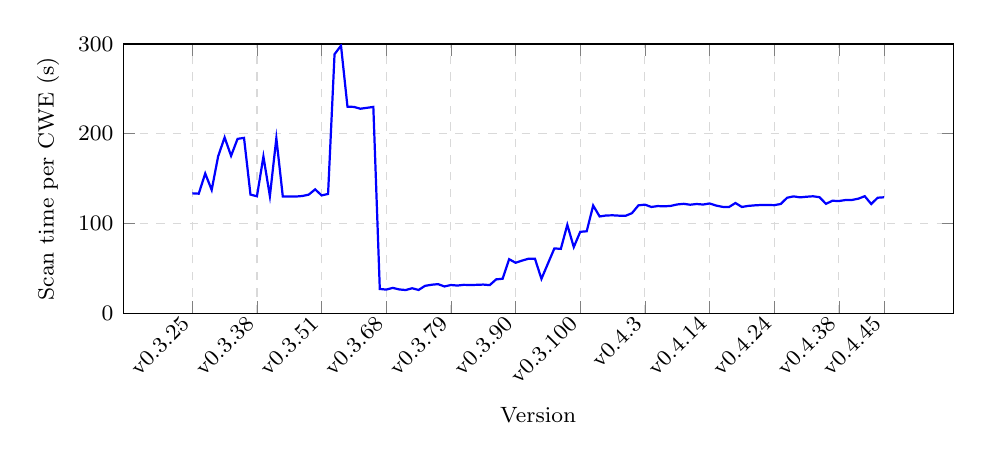
\begin{tikzpicture}
\begin{axis}[
    width=\columnwidth,
    height=5cm,
    xlabel={Version},
    ylabel={Scan time per CWE (s)},
    ymin=0, ymax=300,
    xtick={1, 11, 21, 31, 41, 51, 61, 71, 81, 91, 101, 108},
    xticklabels={v0.3.25, v0.3.38, v0.3.51, v0.3.68, v0.3.79, v0.3.90, v0.3.100, v0.4.3, v0.4.14, v0.4.24, v0.4.38, v0.4.45},
    xticklabel style={rotate=45, anchor=east, font=\footnotesize},
    ylabel style={font=\footnotesize},
    xlabel style={font=\footnotesize},
    tick label style={font=\footnotesize},
    grid=major,
    grid style={dashed, gray!30},
]
\addplot[color=blue, thick, mark=none] coordinates {
    (1, 133.6) (2, 133.2) (3, 155.7) (4, 137.4) (5, 174.9) (6, 195.9) (7, 175.4) (8, 194.3) (9, 195.4) (10, 132.2) (11, 130.3) (12, 174.6) (13, 130.5) (14, 195.0) (15, 130.0) (16, 130.0) (17, 130.0) (18, 130.6) (19, 132.1) (20, 138.0) (21, 131.3) (22, 132.9) (23, 288.6) (24, 298.2) (25, 230.2) (26, 229.9) (27, 227.9) (28, 228.9) (29, 229.9) (30, 27.0) (31, 26.3) (32, 28.2) (33, 26.5) (34, 25.8) (35, 27.8) (36, 25.9) (37, 30.5) (38, 31.7) (39, 32.4) (40, 29.8) (41, 31.4) (42, 30.8) (43, 31.6) (44, 31.4) (45, 31.6) (46, 31.9) (47, 31.3) (48, 37.7) (49, 38.4) (50, 60.2) (51, 56.2) (52, 58.6) (53, 60.7) (54, 60.6) (55, 38.3) (56, 55.3) (57, 72.2) (58, 71.7) (59, 98.5) (60, 73.7) (61, 90.7) (62, 91.3) (63, 120.0) (64, 107.8) (65, 108.9) (66, 109.1) (67, 108.7) (68, 108.5) (69, 111.5) (70, 120.2) (71, 121.0) (72, 118.4) (73, 119.4) (74, 119.1) (75, 119.6) (76, 121.2) (77, 121.9) (78, 120.9) (79, 121.7) (80, 121.1) (81, 122.3) (82, 120.0) (83, 118.5) (84, 118.3) (85, 122.8) (86, 118.4) (87, 119.6) (88, 120.2) (89, 120.6) (90, 120.6) (91, 120.4) (92, 121.7) (93, 128.7) (94, 130.2) (95, 129.1) (96, 129.8) (97, 130.3) (98, 129.3) (99, 121.9) (100, 125.3) (101, 125.0) (102, 126.1) (103, 126.2) (104, 127.6) (105, 130.4) (106, 121.7) (107, 128.7) (108, 129.2)
};
\end{axis}
\end{tikzpicture}
\caption{Juliet scan time per CWE across 108 released versions
(v0.3.25--v0.4.45). The metric is the summed
per-CWE \texttt{sqc} analysis time divided by the number of CWEs scanned,
making it independent of both parallelism (\texttt{--jobs}) and corpus growth
(68--74 CWEs). The sharp drop at v0.3.67 is a single perf optimization
($\approx$8$\times$); the subsequent climb is the cost of added
inter-procedural analysis, which still settles below the v0.3.5x peak.}
\label{fig:scan-time}
\end{figure}

